\documentclass{thomasClass}
\usepackage{amssymb}

\title{\textbf{Required Practical 2}
\\Preparation of stained squashes of cells from plant root tips; set up and use of and optical microscope to identify the stages of mitosis in these stained squashes and calculation of a mitotic index
}
\author{Thomas Boxall}
\date{December 2020}

\begin{document}

\maketitle

\section{Method}
\begin{enumerate}
    \item Take fresh root tip from garlic clove which has been suspended over water and put in 1M hydrochloric acid for 5 minutes at 60\textdegree C.
    \item Rinse the roots under cold water
    \item Submerge the root tips in the stain - acetic orcein. Put this in the water bath for 5 minutes at 60\textdegree C.
    \item Take the root tip out of the stain then place on a microscope slide.
    \item Add a drop of water to the root tip on the slide.
    \item Tease the root tip with a mounted needle to spread the cells apart.
    \item Put a cover slip over the root tip.
    \item Wrap the slide in several layers of paper towels, and squish. Put this under the microscope and view.
\end{enumerate}

\section{Graticule calculations}
Length of cell = 0.4 AU at 400X magnification \\
1mm = 10AU at 100X \\
1AU = 0.1mm \\
$\therefore 0.1AU - 0.01mm$\\
$\therefore 0.4AU = 0.04mm$

\section{Risk assessment}
\begin{table}[H]
    \centering
    \begin{tabularx}{\textwidth}{X|X|X}
        Hazard & Risk & Control\\
        \hline
        Chemicals (incl. acid) & Spilling chemicals onto human flesh; spilling chemicals into eyes & Handle with care; wear safety glasses \\
        Glass slide & When squashing, slide could shatter & Wrap slide in paper towel before squashing
    \end{tabularx}
\end{table}

\section{Diagram}
\begin{figure}[H]
    \centering
    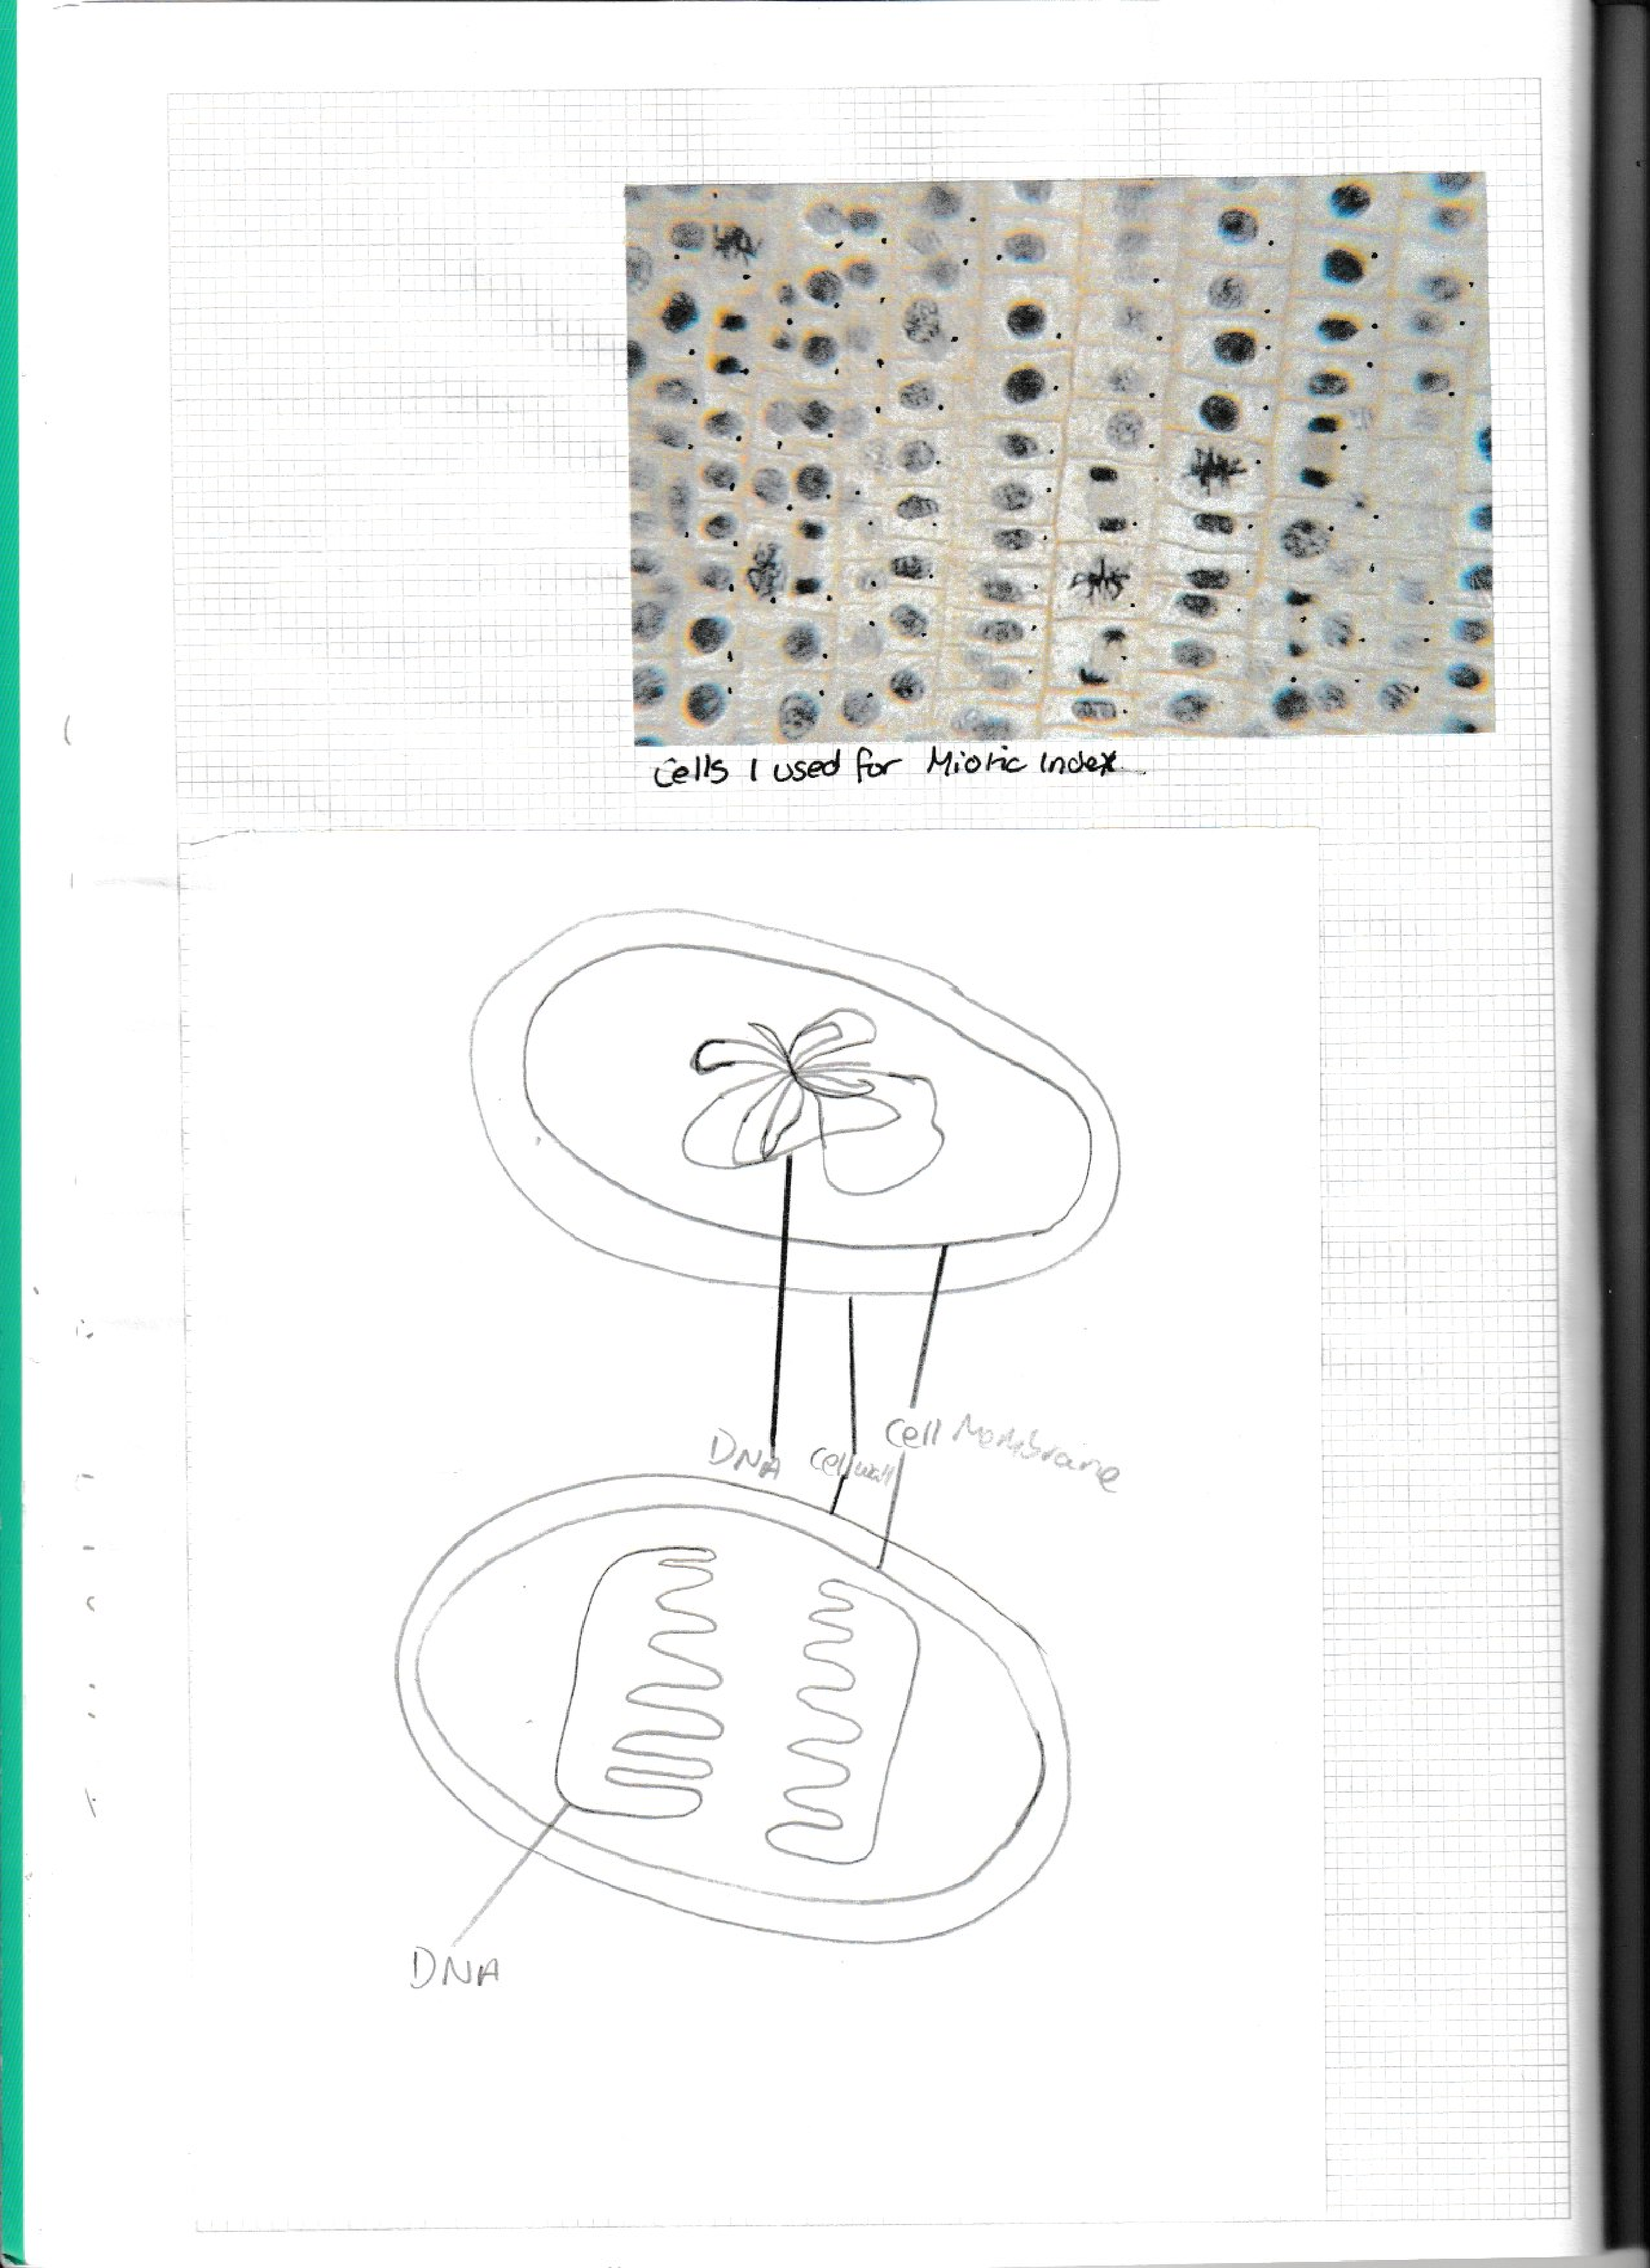
\includegraphics[width=0.9\textwidth]{RPA2-IMAGE.pdf}
    \caption{Drawn diagram of cells undergoing mitosis and cells used for calculating the miotic index}
    \label{fig:RPA-2-IMAGE}
\end{figure}

\section{Miotic index}
Total cells = 86\\
Undergoing Mitosis = 8\\
Miotic Index = $\frac{8}{86}\times 100 = 9.3\%$
\end{document}
